\section{Bilder}
\subsection{Einfaches Bild volle Textbreite}\label{sec:images-textwidth}

\begin{figure}[!ht]
    \centering
    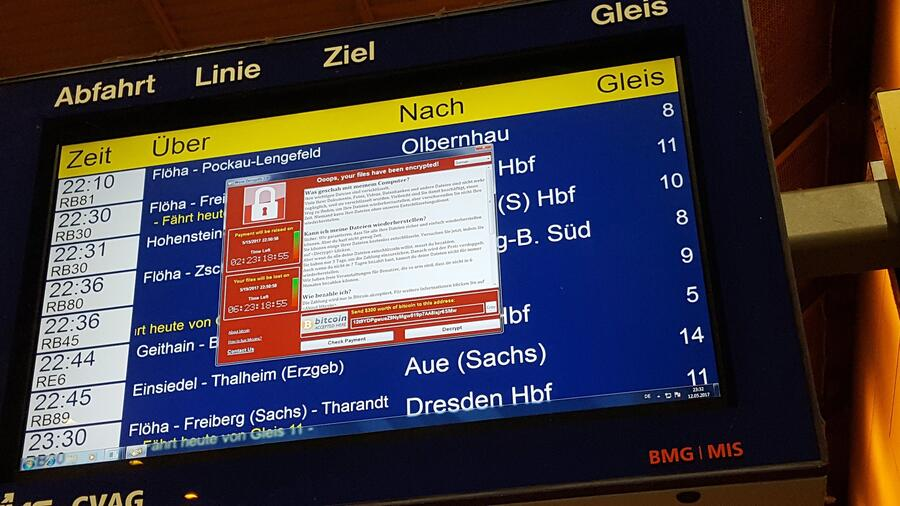
\includegraphics[width=1.0\textwidth]{images/example}
    \caption{\label{fig:example}Beispielbild\protect
    }
\end{figure}

In der Abbildung~\ref{fig:example} ist ein Beispielbild zu sehen.
Bilder werden mit \lstinline|\begin{figure}| eingeleitet.
Mit \lstinline|\includegraphics[width=1.0\textwidth]{Pfad/zum/Bild}| wird 
das Bild hinzugefügt, wobei das Bild durch die Zahl skaliert werden kann.
Das Pfad/zum/Bild ist mit dem relationalen Pfad zum Bild vom Projektordner aus zu ersetzen. 


\subsection{Mehrere Bilder nebeneinander}\label{sec:images-multiple}
\begin{figure}[!htb]
    \centering
    \hyperref[fig:big-example]{
    \minipage{0.46\textwidth}
        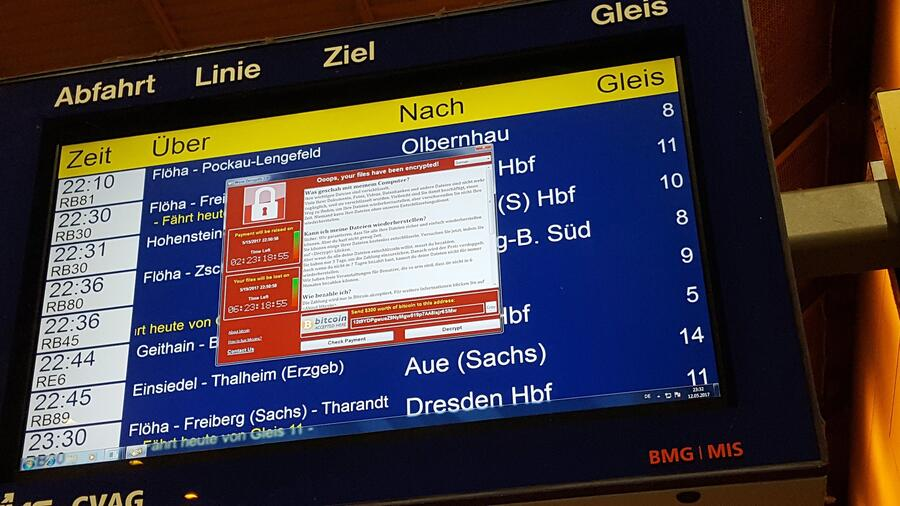
\includegraphics[width=\linewidth]{images/example}
        \caption{\label{fig:example-a}Beispielbild A}
    \endminipage\hfill
    }
    \hyperref[fig:big-example]{
    \minipage{0.46\textwidth}
        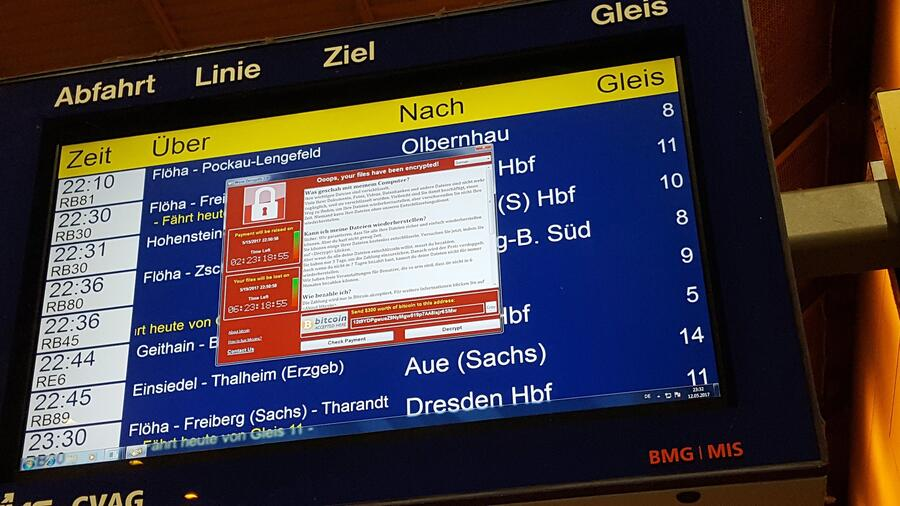
\includegraphics[width=\linewidth]{images/example}
        \caption{\label{fig:example-b}Beispielbild B}
    \endminipage\hfill
    }
    \hyperref[fig:big-example]{
    \minipage{0.46\textwidth}
        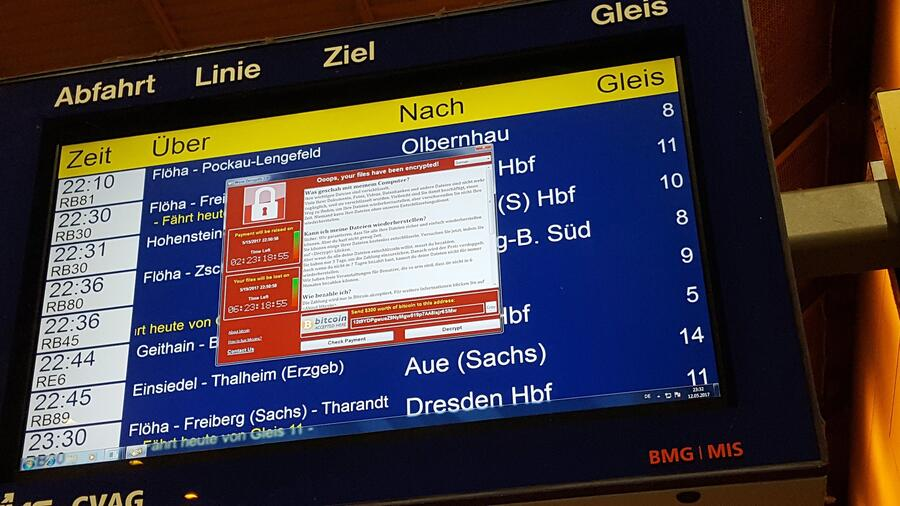
\includegraphics[width=\linewidth]{images/example}
        \caption{\label{fig:example-c}Beispielbild C}
    \endminipage\hfill
    }
    \hyperref[fig:big-example]{
    \minipage{0.46\textwidth}
        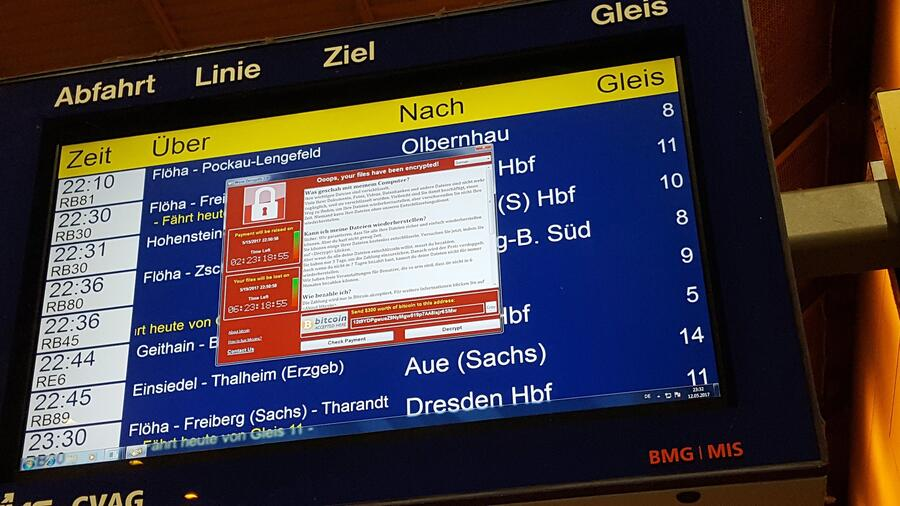
\includegraphics[width=\linewidth]{images/example}
        \caption{\label{fig:example-d}Beispielbild D}
    \endminipage\hfill
    }
    \caption{\label{fig:example-collection}Kollektion}
\end{figure}

In der \nameref{fig:example-collection} von Bildern in Abbildung~\ref{fig:example-collection}
ist die zusammenhängende Darstellung von Bildern gezeigt.
Die Bilder sind in den Anhang verlinkt. Wenn auf ein Bild geklickt wird, kann dieses 
in voller Größe im Anhang betrachtet werden.
Die Verlinkung ist in \path{attachments\bigpicture.tex} zu sehen.


\section{Tabellen}
\begin{table}[ht]
    \centering
    \begin{tabular}{ l c r }
        \toprule
                                & BIOS              & UEFI              \\
        \toprule
        \toprule
        Standardisiert          & Nein              & Ja                \\
        \midrule
        \midrule
        Aktualisierbar          & Nein              & Ja                \\
        \midrule
        \midrule
        Programmiersprache      & Assembler         & C                 \\
                                & schwer lesbar     & einfacher lesbar  \\
        \midrule
        \midrule
        Prozessormodus          & 16 Bit            & 32-64 Bit         \\
        Modulumsetzung          & Option-ROM        & Treiber           \\
        Parallele Ausführung    & Nein              & Ja                \\
        Geschwindigkeit         & Langsamer         & Schneller         \\
        \midrule
        \midrule
        \multicolumn{3}{l}{Verwendete Formatierung der Festplatten}\\
        \midrule
                                & MBR               & GPT               \\
                                & max 4 Partitionen & unlimitiert Partitionen\\
                                & max 2.1TB/HDD     & max 9.44ZB/HDD    \\
        \bottomrule
    \end{tabular}
    \caption{Vergleich von BIOS und UEFI}\label{tab:bios_uefi}
\end{table}

In Tabelle~\ref{tab:bios_uefi} ist ein Beispiel für eine Tabelle zu sehen.
Die Anzahl der Spalten wird nach \lstinline|\begin{tabular}| definiert.
Hier wird gleichzeitig auch die Textausrichtung mit c(=center),l(=left) oder r(=right) gesetzt werden. 
Die einzelnen Zellen der Tabelle werden mit \& voneinander getrennt und mit \lstinline|\\| beendet.
Mehrere Spalten können mit \lstinline|\multicolumn{x}{y}{Text}| verbunden werden,
wobei x die Anzahl der zusammengeführten Spalten und y die Textausrichtung (l, c oder r) ist.


\section{Listings}
\begin{lstlisting}[caption={HelloWorld Programm in Python},captionpos={b},label={lst:helloworld-python},language={Python}] 
    def main():
        print("Hello World\n");
        
    main()
\end{lstlisting}

Listings enthalten Quellcode von Programmen.
Das Beispiel in Listing~\ref{lst:helloworld-python} veranschaulicht das \nameref{lst:helloworld-python}.
Bei \lstinline|\begin{lstlisting}| sind in den eckigen Klammern folgende Eigenschaften definiert.
\begin{description}
    \item[caption] beinhaltet die Beschreibung des Listing
    \item[captionpos] positioniert die Beschreibung unter das Listing.
    \item[label] wird verwendet, um das Listing mit \lstinline|~\ref{lst:...}| im Text referenzieren zu können.
    \item[language] ist die Programmiersprache, die für das Markup verwendet wird.
\end{description}
Folgende Programmiersprachen sind im \lstinline|language|-Feld der Listings möglich.\\
ABAP2,4, ACSL, Ada4, Algol4, Ant, Assembler2,4, Awk4, bash, Basic2,4, C\#5, C++4, C4, Caml4, Clean, 
Cobol4, Comal, csh, Delphi, Eiffel, Elan, erlang, Euphoria, Fortran4, GCL, Go (golang), Gnuplot, Haskell, 
HTML, IDL4, inform, Java4, JVMIS, ksh, Lisp4, Logo, Lua2, make4, Mathematica1,4, Matlab, Mercury, MetaPost, 
Miranda, Mizar, ML, Modelica3, Modula-2, MuPAD, NASTRAN, Oberon-2, Objective C5 , OCL4, Octave, Oz, Pascal4, 
Perl, PHP, PL/I, Plasm, POV, Prolog, Promela, Python, R, Reduce, Rexx, RSL, Ruby, S4, SAS, Scilab, sh, SHELXL, 
Simula4, SQL, tcl4, TeX4, VBScript, Verilog, VHDL4, VRML4, XML, XSLT\footnote{Website mit unterstützten Programmiersprachen für Listings}. 
